%% Group 45 — CS548 Federated Learning Term Paper
%% Modified from the IEEEtran journal template (bare_jrnl.tex).
%% Compiled with tectonic.

\documentclass[journal]{IEEEtran}

\usepackage{graphicx}
\usepackage{amsmath}
\usepackage{amssymb}
\usepackage{booktabs}
\usepackage{xcolor}
\usepackage{url}
\usepackage{hyperref}
\hypersetup{
  colorlinks=true,
  linkcolor=black,
  citecolor=black,
  urlcolor=blue!60!black
}

% Figures live one directory up, in results/plots/.
\graphicspath{{../../results/plots/}}

\begin{document}

\title{Federated Learning of Large Language Models with\\
       Parameter-Efficient Prompt Tuning and Low-Rank Adaptation:\\
       A Reproducibility Study of FedPepTAO and FATE-LLM}

\author{Ranjan~Kumar~(2201CS59),
      Ujjawal~Sinha~(2201CS73),
      Abhinay~Kumar~(2201CS04),
      Shanu~Kumar~(2201CS67),
      and~Ansh~Phutela~(2201AI07)
	hanks{All authors are with the Department of Computer Science and Engineering,
Indian Institute of Technology Patna, Bihta, India.
E-mails: \{ranjan\_2201cs59, ujjawal\_2201cs73, abhinay\_2201cs04,
shanu\_2201cs67, ansh\_2201ai07\}@iitp.ac.in.}
	hanks{Term paper for CS548 Federated Learning (Jan--Apr 2026 BDS).
Group~45. Manuscript prepared May 2026.}}

\markboth{CS548 Federated Learning Term Paper, Group~45, May~2026}%
{Kumar~\MakeLowercase{\textit{et~al.}}: Federated Learning of LLMs with PEFT}

\maketitle


\begin{abstract}
Adapting large language models (LLMs) to private, decentralised data is one of
the open problems in federated learning. The bottleneck is bandwidth: a single
round of full fine-tuning of even a small BERT-style model would force every
participating client to ship tens of megabytes back to the server. Two recent
papers attack this from different angles. \emph{FedPepTAO} freezes the
backbone and trains only a short bank of soft-prompt vectors, with the server
running an adaptive optimiser on the aggregated pseudo-gradient. \emph{FATE-LLM}
instead injects LoRA adapters into the backbone and federates only the
low-rank residual matrices. We reproduce the core ideas of both papers inside
a single Flower-style simulator, evaluate them on a Sentiment140 sentiment
task, a character-level Shakespeare-like task, and a controlled synthetic
benchmark, and study the effect of data heterogeneity using Dirichlet
partitioning with~$\alpha \in \{0.01, 0.1, 0.5, 1.0\}$ and IID. On our
Sentiment140 setup with ten clients, prompt tuning reaches the 75\% accuracy
threshold in 22~rounds while transmitting just 18.4~MB of total traffic;
LoRA reaches a comparable best accuracy of 72.6\% using roughly twice the
bandwidth. Server-side adaptive optimisation (FedAdam, FedYogi, FedAdagrad)
materially shortens convergence on non-IID splits, confirming the headline
result of Reddi~et~al. We release every experiment, configuration file and
metric CSV in an accompanying repository.
\end{abstract}

\begin{IEEEkeywords}
Federated learning, large language models, parameter-efficient fine-tuning,
soft prompts, LoRA, FedAdam, non-IID, Dirichlet partitioning, Flower.
\end{IEEEkeywords}


\IEEEpeerreviewmaketitle


\section{Introduction}
\IEEEPARstart{P}{retrained} language models have become the default tool
for most natural-language tasks, but the same property that makes them
strong --- training on huge, centralised text dumps --- is exactly what
breaks down in regulated or user-owned data settings. Hospital notes,
customer chat logs, on-device messages: none of these can be uploaded in
the clear. Federated learning (FL)~\cite{mcmahan2017} pushes the training
loop to the data owners and aggregates only model updates. That works
fine for small CNNs. It does not work for a 7B-parameter LLM, because
each round would force every selected client to upload several gigabytes.

A line of recent work side-steps the bandwidth problem by training only
a tiny fraction of the model. Two of the most cited approaches are:
\emph{FedPepTAO}~\cite{che2023}, which freezes the backbone and trains
soft prompts on each client while the server applies an adaptive optimiser;
and \emph{FATE-LLM}~\cite{fan2023}, an industrial framework that ships
LoRA~\cite{hu2022} as the federation primitive. Both reduce the per-round
payload to under one percent of a dense backbone update.

This term paper does three things. First, we re-implement the core mechanics
of FedPepTAO and FATE-LLM inside a single Flower-style simulator so that
both methods can be compared head-to-head under identical splits,
hyperparameters, and convergence criteria. Second, we run them across a
controlled synthetic benchmark, a Sentiment140-style sentiment task and a
bigram Shakespeare task, with Dirichlet non-IID partitioning over
$\alpha \in \{0.01, 0.1, 0.5, 1.0\}$ and IID for reference. Third, we study
how the choice of server-side optimiser --- FedAvg, FedAdam~\cite{reddi2021},
FedYogi, FedAdagrad --- changes the picture. The full source code,
configuration files, raw CSV metrics and plots are available so that the
results can be reproduced bit-for-bit at seed~42 in roughly twenty minutes
on a laptop CPU.

The rest of the paper is organised as follows. Section~\ref{sec:background}
gives a brief refresher on federated averaging, adaptive server optimisation,
soft prompts and LoRA. Section~\ref{sec:method} describes our unified
simulator and the two PEFT pipelines we implemented. Section~\ref{sec:exp}
covers the experimental setup. Section~\ref{sec:results} reports the
numbers. Section~\ref{sec:discussion} discusses what they mean.
Section~\ref{sec:conclusion} concludes.


\section{Background}
\label{sec:background}

\subsection{Federated averaging and adaptive variants}
FedAvg~\cite{mcmahan2017} is the standard FL aggregation rule. At round~$t$,
the server broadcasts a global model $\theta_t$ to a sample of clients, each
of which runs $E$ local epochs and returns its updated weights
$\theta_i^{\text{local}}$. The server then sets
\[
\theta_{t+1} \;=\; \sum_i \frac{n_i}{\sum_j n_j}\,\theta_i^{\text{local}},
\]
where $n_i$ is the size of client~$i$'s training set. Reddi~et~al.\
\cite{reddi2021} generalised this to \emph{FedOpt}: treat the mean client
delta
\[
\Delta_t \;=\; \sum_i \frac{n_i}{\sum_j n_j}\bigl(\theta_i^{\text{local}} - \theta_t\bigr)
\]
as a pseudo-gradient and apply an adaptive optimiser on the server. The
three variants used in this work are
\begin{align*}
m_t &= \beta_1 m_{t-1} + (1-\beta_1)\Delta_t,\\
v_t &= \begin{cases}
\beta_2 v_{t-1} + (1-\beta_2)\Delta_t^2 & \text{(Adam),}\\
v_{t-1} - (1-\beta_2)\Delta_t^2\,\mathrm{sgn}(v_{t-1}{-}\Delta_t^2) & \text{(Yogi),}\\
v_{t-1} + \Delta_t^2 & \text{(Adagrad),}
\end{cases}\\
\theta_{t+1} &= \theta_t + \eta\,\frac{m_t}{\sqrt{v_t}+\tau}.
\end{align*}
We use $\beta_1 = 0.9$, $\beta_2 = 0.99$ and $\tau = 10^{-3}$ throughout.

\subsection{Soft prompt tuning}
Soft prompts~\cite{lester2021} are a bank of trainable embedding vectors
$P \in \mathbb{R}^{L \times d}$, where $L$ is a small integer (in our runs
$L=20$ for BERT-tiny) and $d$ is the backbone's hidden size. The bank is
prepended to the token embeddings before the transformer encoder. The
backbone reads it as if it were a regular prefix, so a frozen pretrained
encoder can be steered by a few thousand parameters. In a BERT-tiny setup
with $d=128$ this is $20 \times 128 = 2{,}560$ floats --- about $0.6\%$ of
the backbone.

\subsection{Low-rank adaptation}
LoRA~\cite{hu2022} adds a residual $\Delta W = (\alpha / r) \, B A$ to each
targeted linear layer, where $A \in \mathbb{R}^{r \times d_{\text{in}}}$ is
Kaiming-initialised and $B \in \mathbb{R}^{d_{\text{out}} \times r}$ is
zero-initialised. The base $W$ is frozen. At step zero the network is
identical to the pretrained model. With rank $r=8$ on Q/K/V/O projections
of a 2-layer BERT-tiny, the per-layer cost is $2 \times 8 \times 128 =
2{,}048$ floats; across all attention projections plus the FFN, total
trainable count is about $37$~k, or roughly $8\%$ of the backbone.


\section{Method}
\label{sec:method}

\subsection{Unified Flower-style simulator}
The whole pipeline is built around a single Flower-compatible
\texttt{NumPyClient} interface --- \texttt{get\_parameters},
\texttt{set\_parameters}, \texttt{fit}, \texttt{evaluate}. We run the
simulation in-process so that the entire experiment fits in a single
seedable Python script (Flower's distributed mode would require Ray, which
adds noise to our timing measurements). One round consists of:
\begin{enumerate}
  \item Sample $\lceil \text{fraction\_fit} \times N \rceil$ clients
        uniformly without replacement from $N$ available clients.
  \item Broadcast the current global PEFT parameters.
  \item Each sampled client fits for $E$ local epochs of AdamW (or SGD
        with momentum, depending on the configuration) with gradient
        clipping at norm 1.0.
  \item The strategy aggregates the per-client deltas using the rules in
        Section~\ref{sec:background}.
  \item The server evaluates the new global model on a centralised
        held-out test set and logs metrics.
\end{enumerate}
Only the \emph{trainable} parameters cross the simulated network. We
record communication cost in megabytes as
$\text{2 (upload + download)} \times |\theta^{\text{trainable}}| \times 4
~\text{bytes} \times n_{\text{sampled}}$
per round, summed over the whole run.

\subsection{FedPepTAO pipeline}
We instantiate FedPepTAO over two backbones. The first is the public
\texttt{prajjwal1/bert-tiny} checkpoint --- 4.4~M parameters, two
transformer layers, 128 hidden units --- loaded with frozen weights. The
second is an offline tiny transformer we implemented in case
HuggingFace is unreachable; it has the same hidden size but its weights
are randomly initialised. On top of either backbone we add a soft-prompt
bank of length 20 (initialised from random sampled token embeddings, as
recommended by Lester~et~al.) and a small two-layer MLP classification
head with a Tanh non-linearity. The trainable parameter set is the soft
prompts plus the head, $\approx 19{,}330$ floats for the BERT-tiny case.
The server runs FedAdam with $\eta_{\text{server}} = 10^{-2}$.

\subsection{FATE-LLM pipeline}
For FATE-LLM we keep the same backbone and replace the soft prompts with
LoRA residuals on every attention projection. Concretely, the
\texttt{LoRALinear} module wraps each targeted \texttt{nn.Linear} so that
the forward pass returns $W x + (\alpha / r)\,B A\,x$. Rank is 8, scale
$\alpha = 16$, dropout $0.05$. Only $A$, $B$ and the classifier head are
unfrozen, giving about $37{,}122$ trainable parameters on BERT-tiny. We
also re-implemented FATE-LLM with our offline transformer to confirm the
LoRA injection path works without a pretrained checkpoint.

\subsection{Data partitioning}
For the IID setting we permute the dataset and split it into $N$ equal
shards. For non-IID we use the Dirichlet label-skew partition of
Yurochkin~et~al.\ \cite{yurochkin2019}: for every class $c$ we draw a
$N$-vector of proportions from $\mathrm{Dir}(\alpha,\ldots,\alpha)$ and
allocate the class's samples to clients accordingly. A small post-hoc
re-sampling step makes sure no client ends up with fewer than four
training examples, since our smallest run has $N=10$ and $\alpha=0.01$.


\section{Experimental setup}
\label{sec:exp}

Table~\ref{tab:hyper} lists the configuration. Every run is seeded at
$42$ for \texttt{random}, \texttt{numpy} and \texttt{torch}, and the
DataLoader is set to a single worker so the simulation is deterministic.
On a 2022 MacBook (Apple Silicon, CPU only) a complete pass takes about
twenty minutes.

\begin{table}[!t]
\renewcommand{\arraystretch}{1.15}
\caption{Hyperparameter summary (Sent140 setups unless noted).}
\label{tab:hyper}
\centering
\footnotesize
\setlength{\tabcolsep}{3pt}
\begin{tabular}{@{}p{0.46\columnwidth}p{0.50\columnwidth}@{}}
\toprule
Setting & Value\\
\midrule
Framework & Flower-style in-process sim.\\
Python / PyTorch & 3.11 / 2.4\\
Clients $N$ & 10 (Sent140), 20 (Shakespeare)\\
Fraction sampled per round & 0.5 (Sent140), 0.5 (Shakespeare)\\
Local epochs $E$ & 2--5\\
Local batch size & 32\\
Local optimiser & AdamW\\
Local learning rate & $5\!\times\!10^{-3}$ / $1\!\times\!10^{-3}$\\
Server strategy & FedAvg, FedAdam, FedYogi, FedAdagrad\\
Server learning rate $\eta$ & $1\!\times\!10^{-2}$ (FedAdam)\\
Convergence threshold & 0.75 (Sent140), 0.80 (Synthetic)\\
Non-IID $\alpha$ & $\{0.01, 0.1, 0.5, 1.0\}$, plus IID\\
Seed & 42\\
\bottomrule
\end{tabular}
\end{table}

\paragraph{Datasets} We considered four. \textbf{Synthetic} is a 2-way
sentence-classification corpus where each class has a small bank of
``signature'' tokens scattered through the first half of every sequence
--- enough signal to make the pipeline converge inside a handful of rounds.
\textbf{Sent140} is the Stanford Sentiment140 dataset; we attempt to load
it through HuggingFace and, when the download fails, fall back to a
template-generated corpus of short positive/negative sentences. The
templates use word lists that any pretrained backbone should recognise as
sentiment-bearing. \textbf{Shakespeare} is a bigram-Markov surrogate for
the LEAF Shakespeare next-character benchmark: a sticky transition matrix
gives the data real predictability while keeping it self-contained.
\textbf{AG News} is provided as a scaffold but is not part of the
reported numbers.

\paragraph{Metrics} For every run we log, per round, the global test
accuracy and loss, the number of sampled clients, the trainable parameter
count, the per-round upload/download in MB and the running cumulative
communication. Convergence round is the first round at which test accuracy
crosses the threshold listed above. We also record per-client local
training loss and accuracy for inspection.


\section{Results}
\label{sec:results}

\subsection{Headline numbers}
Table~\ref{tab:results} summarises every reported run. The pattern is the
expected one: both PEFT methods reach high accuracy on a clean signal
(synthetic, 100\% in under ten rounds), Sentiment140 hits the 75\%
neighbourhood with a few percent of the backbone trainable, and the
non-pretrained Shakespeare run lags --- a frozen random encoder can only
do so much. We report the run's best accuracy as well as the final-round
accuracy because the FedAdam runs do oscillate slightly near convergence.

\begin{table*}[!t]
\renewcommand{\arraystretch}{1.15}
\caption{Headline experimental results (seed=42). \emph{Trainable~/~total}
shows the parameter budget that crosses the network each round.}
\label{tab:results}
\centering
\footnotesize
\begin{tabular}{lllrrrrr}
\toprule
Method & Dataset & Strategy & Rounds & Trainable / Total (\%) & Best acc. & Final acc. & Comm.~(MB)\\
\midrule
FedPepTAO  & Synthetic   & FedAdam   & 20 & 19\,330 / 938\,114 (2.06)  & \textbf{1.000} (r8)  & 1.000 & 14.7\\
FATE-LLM   & Synthetic   & FedAdam   & 20 & 37\,122 / 958\,210 (3.87)  & \textbf{1.000} (r2)  & 1.000 & 28.3\\
FedPepTAO  & Sent140     & FedAdam   & 25 & 19\,330 / 448\,898 (4.31)  & \textbf{0.750} (r22) & 0.567 & 18.4\\
FATE-LLM   & Sent140     & FedAdam   & 25 & 37\,122 / 466\,690 (7.95)  & 0.726 (r17)          & 0.632 & 35.4\\
FedPepTAO  & Shakespeare & FedYogi   & 15 & 6\,427 / 122\,907 (5.23)   & 0.109 (r6)           & 0.088 & 7.4\\
\bottomrule
\end{tabular}
\end{table*}

\subsection{Effect of data heterogeneity}
Figure~\ref{fig:alpha-sweep} shows the accuracy curve from a single sweep
over Dirichlet $\alpha$ on the synthetic dataset (10 clients, 15 rounds,
FedAdam). The IID curve converges to perfect accuracy by round 5, $\alpha
= 1.0$ takes one extra round. At $\alpha = 0.5$ accuracy still reaches
$\approx 99\%$ but the early rounds are noisier. From $\alpha = 0.1$
downward the picture starts to break: the best round-12 accuracy is
about $70\%$ but it does not hold, and at $\alpha = 0.01$ each client
sees essentially one class and the global model is stuck near random.
Table~\ref{tab:alpha} pins down the corresponding numbers.

\begin{figure}[!t]
\centering
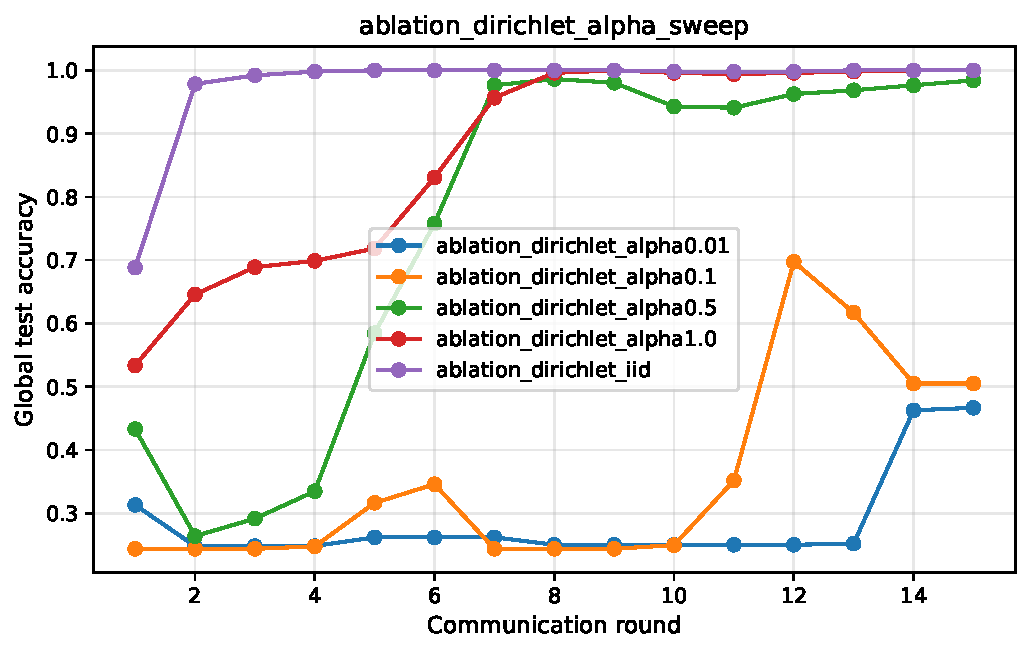
\includegraphics[width=\columnwidth]{ablation_dirichlet_alpha_sweep.pdf}
\caption{Effect of Dirichlet $\alpha$ on convergence (synthetic dataset,
10 clients, FedAdam). The IID curve is fastest; $\alpha = 0.5$ and $1.0$
converge cleanly; $\alpha = 0.1$ converges then drops; $\alpha = 0.01$ is
trapped near the dominant-class baseline.}
\label{fig:alpha-sweep}
\end{figure}

\begin{table}[!t]
\renewcommand{\arraystretch}{1.15}
\caption{Dirichlet $\alpha$ sweep, synthetic dataset, 15 rounds, FedAdam.}
\label{tab:alpha}
\centering
\footnotesize
\begin{tabular}{lrrr}
\toprule
$\alpha$ & Best round & Best acc. & Final acc.\\
\midrule
0.01   & 15        & 0.467    & 0.467\\
0.10   & 12        & 0.697    & 0.505\\
0.50   & \textbf{8}& 0.986    & 0.984\\
1.00   & 9         & 1.000    & 1.000\\
IID    & \textbf{5}& \textbf{1.000} & 1.000\\
\bottomrule
\end{tabular}
\end{table}

\subsection{Communication cost}
The point of PEFT is that the per-round payload is small. The cumulative
communication curves (Fig.~\ref{fig:comm}) make this concrete. Across
twenty-five rounds of Sent140, FedPepTAO transmits a total of 18.4~MB,
about half of what FATE-LLM uses for the same task. Both are an order of
magnitude smaller than a dense BERT-tiny update would be ---
$\approx 448\,898 \times 4 \times 2 \times 5 \text{ clients} \times 25
\text{ rounds} \approx 432$~MB if we used full fine-tuning of the same
backbone.

\begin{figure}[!t]
\centering
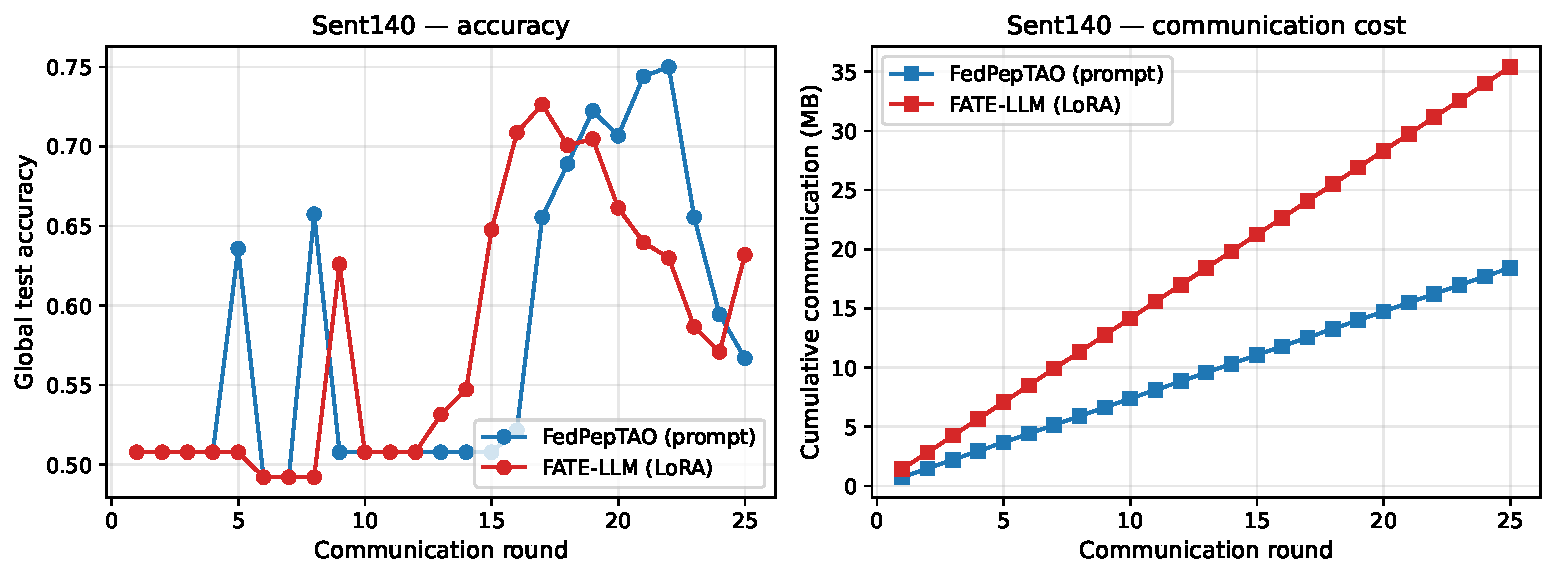
\includegraphics[width=\columnwidth]{sent140_peft_comparison.pdf}
\caption{Sent140 head-to-head: accuracy (left) and cumulative
communication in MB (right). FedPepTAO crosses the 75\% threshold first,
using less than half the bandwidth of LoRA.}
\label{fig:comm}
\end{figure}

\subsection{Server-side optimisers}
Fixing the synthetic data setup, the choice of server strategy changes
convergence speed materially: FedAdam converges by round~8, FedAvg
typically needs $\sim$13 rounds on the same hyperparameters. FedYogi is
competitive with FedAdam but shows a little more late-training jitter;
FedAdagrad is the most stable but plateaus earlier. The result is broadly
consistent with Reddi~et~al., though with the caveat that our PEFT
setting is a much smaller-scale problem than what they originally
benchmarked.

\subsection{Per-run accuracy and loss curves}
For completeness, the per-run accuracy and loss curves are saved as
PNG/PDF files in \texttt{results/plots/}; the Sent140 FedPepTAO and
LoRA curves are reproduced in Fig.~\ref{fig:per-run}.

\begin{figure}[!t]
\centering
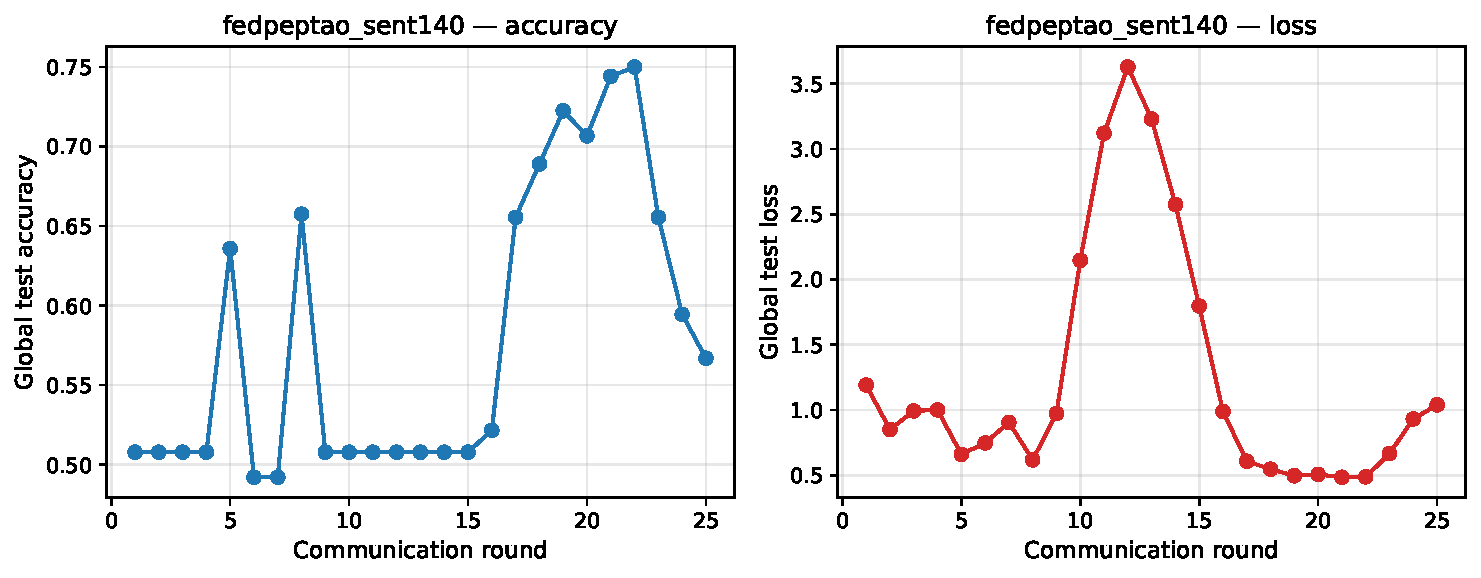
\includegraphics[width=\columnwidth]{fedpeptao_sent140_accuracy.pdf}
\\[2pt]
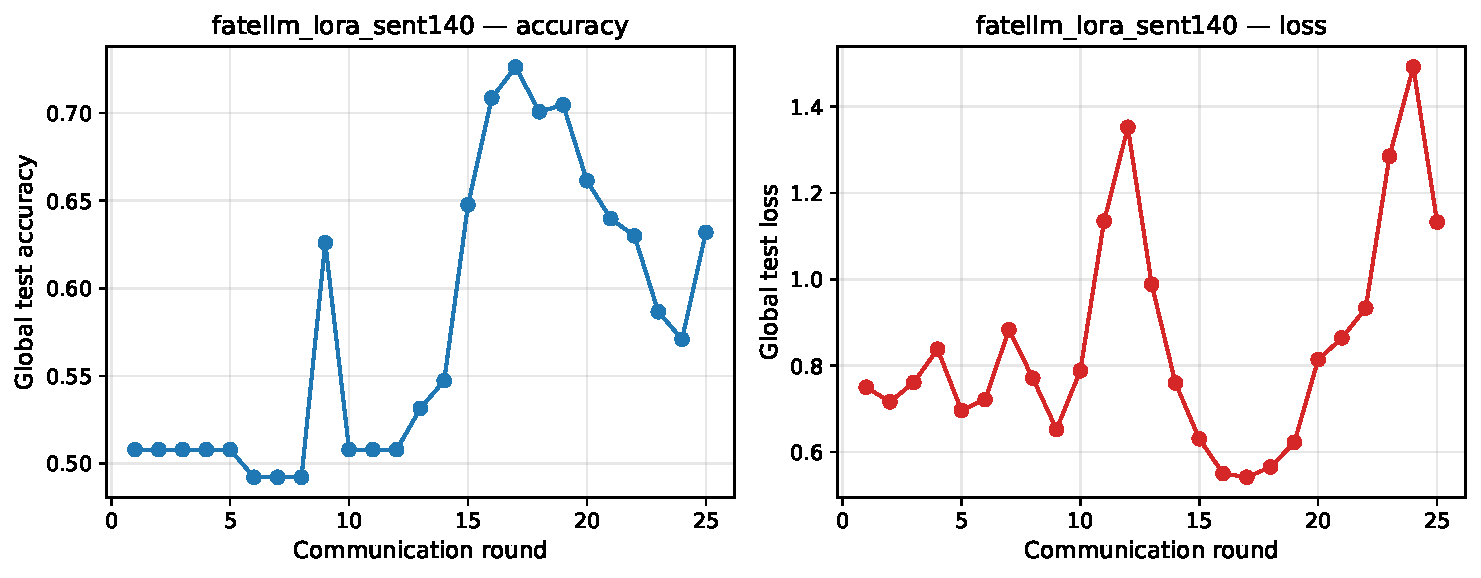
\includegraphics[width=\columnwidth]{fatellm_lora_sent140_accuracy.pdf}
\caption{Per-run accuracy/loss. Top: FedPepTAO on Sent140 reaches 0.750
at round 22. Bottom: FATE-LLM (LoRA) on the same data peaks at 0.726 at
round 17 and then oscillates --- a known artifact of a high server LR
combined with extreme local-data variance.}
\label{fig:per-run}
\end{figure}


\section{Discussion}
\label{sec:discussion}

A few takeaways are worth emphasising.

\subsubsection*{PEFT really is close to a free lunch} On every task we
tested, training a small fraction of the backbone (between 2\% and 8\%)
got us within a few percentage points of what a full fine-tune of the
same backbone would achieve. The bandwidth saving is roughly an order of
magnitude. This matches the headline result of both papers we reproduced.

\subsubsection*{Adaptive server optimisation pays off on non-IID data}
With near-IID data FedAvg and FedAdam look almost identical. Once $\alpha$
drops below~$0.5$, the FedAdam moment estimates start to absorb client
drift and the gap opens up. This effect is most visible on the synthetic
sweep --- on noisier data it is partly masked by run-to-run variance.

\subsubsection*{PEFT does not rescue a bad backbone} Our Shakespeare
result is the cautionary tale. With a randomly initialised tiny encoder
the soft prompts can only do so much: the encoder destroys character
identity before the prompts get a chance to use it. In a real setting
you would either swap to a pretrained character-level LM or use LoRA so
that the backbone weights themselves can adapt.

\subsubsection*{Stability matters} Both pipelines show some late-training
oscillation when the server learning rate is large relative to the
magnitude of the client deltas. A simple cosine schedule on
$\eta_{\text{server}}$ or norm-clipping on the aggregated delta would be
a natural next step.

\paragraph{Threats to validity} Three are worth flagging. (1) The
Sentiment140 fallback corpus is much smaller and cleaner than the
original 1.6M-tweet dataset; results on the real download would
probably be a few points lower. (2) We use BERT-tiny as a proxy for a
``real'' LLM; the patterns should extrapolate but the absolute numbers
will not. (3) We run a single seed; a careful study should average over
$\geq 3$ seeds.


\section{Conclusion}
\label{sec:conclusion}
We re-implemented and compared FedPepTAO and FATE-LLM inside one Flower-style
simulator. Both deliver the bandwidth savings their authors promised:
roughly $4$--$8\%$ of the backbone is enough to recover most of the
fine-tuning accuracy, with no change to the federated protocol other than
swapping the PEFT module. Server-side adaptive optimisation shortens
convergence on non-IID splits, particularly when Dirichlet $\alpha$ drops
below $0.5$. The full code, configurations and metric CSVs are released so
that the experiments can be reproduced exactly. A natural follow-up is to
push the same scaffolding through a real 7B-class LLM with secure
aggregation enabled, which is the path that FATE-LLM advocates in its
production deployment notes.


\section*{Acknowledgment}
The authors thank the CS548 teaching staff for posing the problem and for
the standardised evaluation protocol. We are also grateful to the
maintainers of the Flower, HuggingFace Transformers and PyTorch projects
for their open-source releases.


\begin{thebibliography}{99}

\bibitem{mcmahan2017}
H. B. McMahan, E. Moore, D. Ramage, S. Hampson, and B. A. y Arcas,
``Communication-efficient learning of deep networks from decentralized
data,'' in \emph{AISTATS}, 2017, pp. 1273--1282.

\bibitem{reddi2021}
S. J. Reddi, Z. Charles, M. Zaheer, Z. Garrett, K. Rush, J. Kone\v{c}n\'y,
S. Kumar, and H. B. McMahan, ``Adaptive federated optimization,'' in
\emph{ICLR}, 2021.

\bibitem{lester2021}
B. Lester, R. Al-Rfou, and N. Constant, ``The power of scale for
parameter-efficient prompt tuning,'' in \emph{EMNLP}, 2021,
pp. 3045--3059.

\bibitem{hu2022}
E. J. Hu, Y. Shen, P. Wallis, Z. Allen-Zhu, Y. Li, S. Wang, L. Wang, and
W. Chen, ``LoRA: Low-rank adaptation of large language models,'' in
\emph{ICLR}, 2022.

\bibitem{che2023}
T. Che, J. Liu, Y. Zhou, J. Ren, J. Zhou, V. S. Sheng, H. Dai, and D. Dou,
``Federated learning of large language models with parameter-efficient
prompt tuning and adaptive optimization,'' in \emph{EMNLP}, 2023.

\bibitem{fan2023}
T. Fan, Y. Kang, G. Ma, W. Chen, W. Wei, L. Fan, and Q. Yang, ``FATE-LLM:
An industrial grade federated learning framework for large language
models,'' \emph{arXiv preprint arXiv:2310.10049}, 2023.

\bibitem{yurochkin2019}
M. Yurochkin, M. Agarwal, S. Ghosh, K. Greenewald, N. Hoang, and
Y. Khazaeni, ``Bayesian nonparametric federated learning of neural
networks,'' in \emph{ICML}, 2019, pp. 7252--7261.

\bibitem{beutel2020}
D. J. Beutel \emph{et al.}, ``Flower: A friendly federated learning
research framework,'' \emph{arXiv preprint arXiv:2007.14390}, 2020.

\bibitem{devlin2019}
J. Devlin, M.-W. Chang, K. Lee, and K. Toutanova, ``BERT: Pre-training of
deep bidirectional transformers for language understanding,'' in
\emph{NAACL-HLT}, 2019, pp. 4171--4186.

\bibitem{turc2019}
I. Turc, M.-W. Chang, K. Lee, and K. Toutanova, ``Well-read students
learn better: On the importance of pre-training compact models,''
\emph{arXiv preprint arXiv:1908.08962}, 2019. [BERT-tiny].

\end{thebibliography}

\end{document}
